\documentclass[tikz,border=0pt]{standalone}
\usepackage[american]{circuitikz}
\usetikzlibrary{arrows.meta,calc,positioning,decorations.pathmorphing,patterns}
\definecolor{zyloTeal}{HTML}{174A5B}
\definecolor{zyloTealTwo}{HTML}{246B7A}
\definecolor{zyloInk}{HTML}{1F2933}
\definecolor{zyloSoft}{HTML}{EAF4F4}
\definecolor{zyloPaper}{HTML}{F8FAFB}
\definecolor{zyloLine}{HTML}{44606B}
\definecolor{zyloOrange}{HTML}{D97706}
\begin{document}
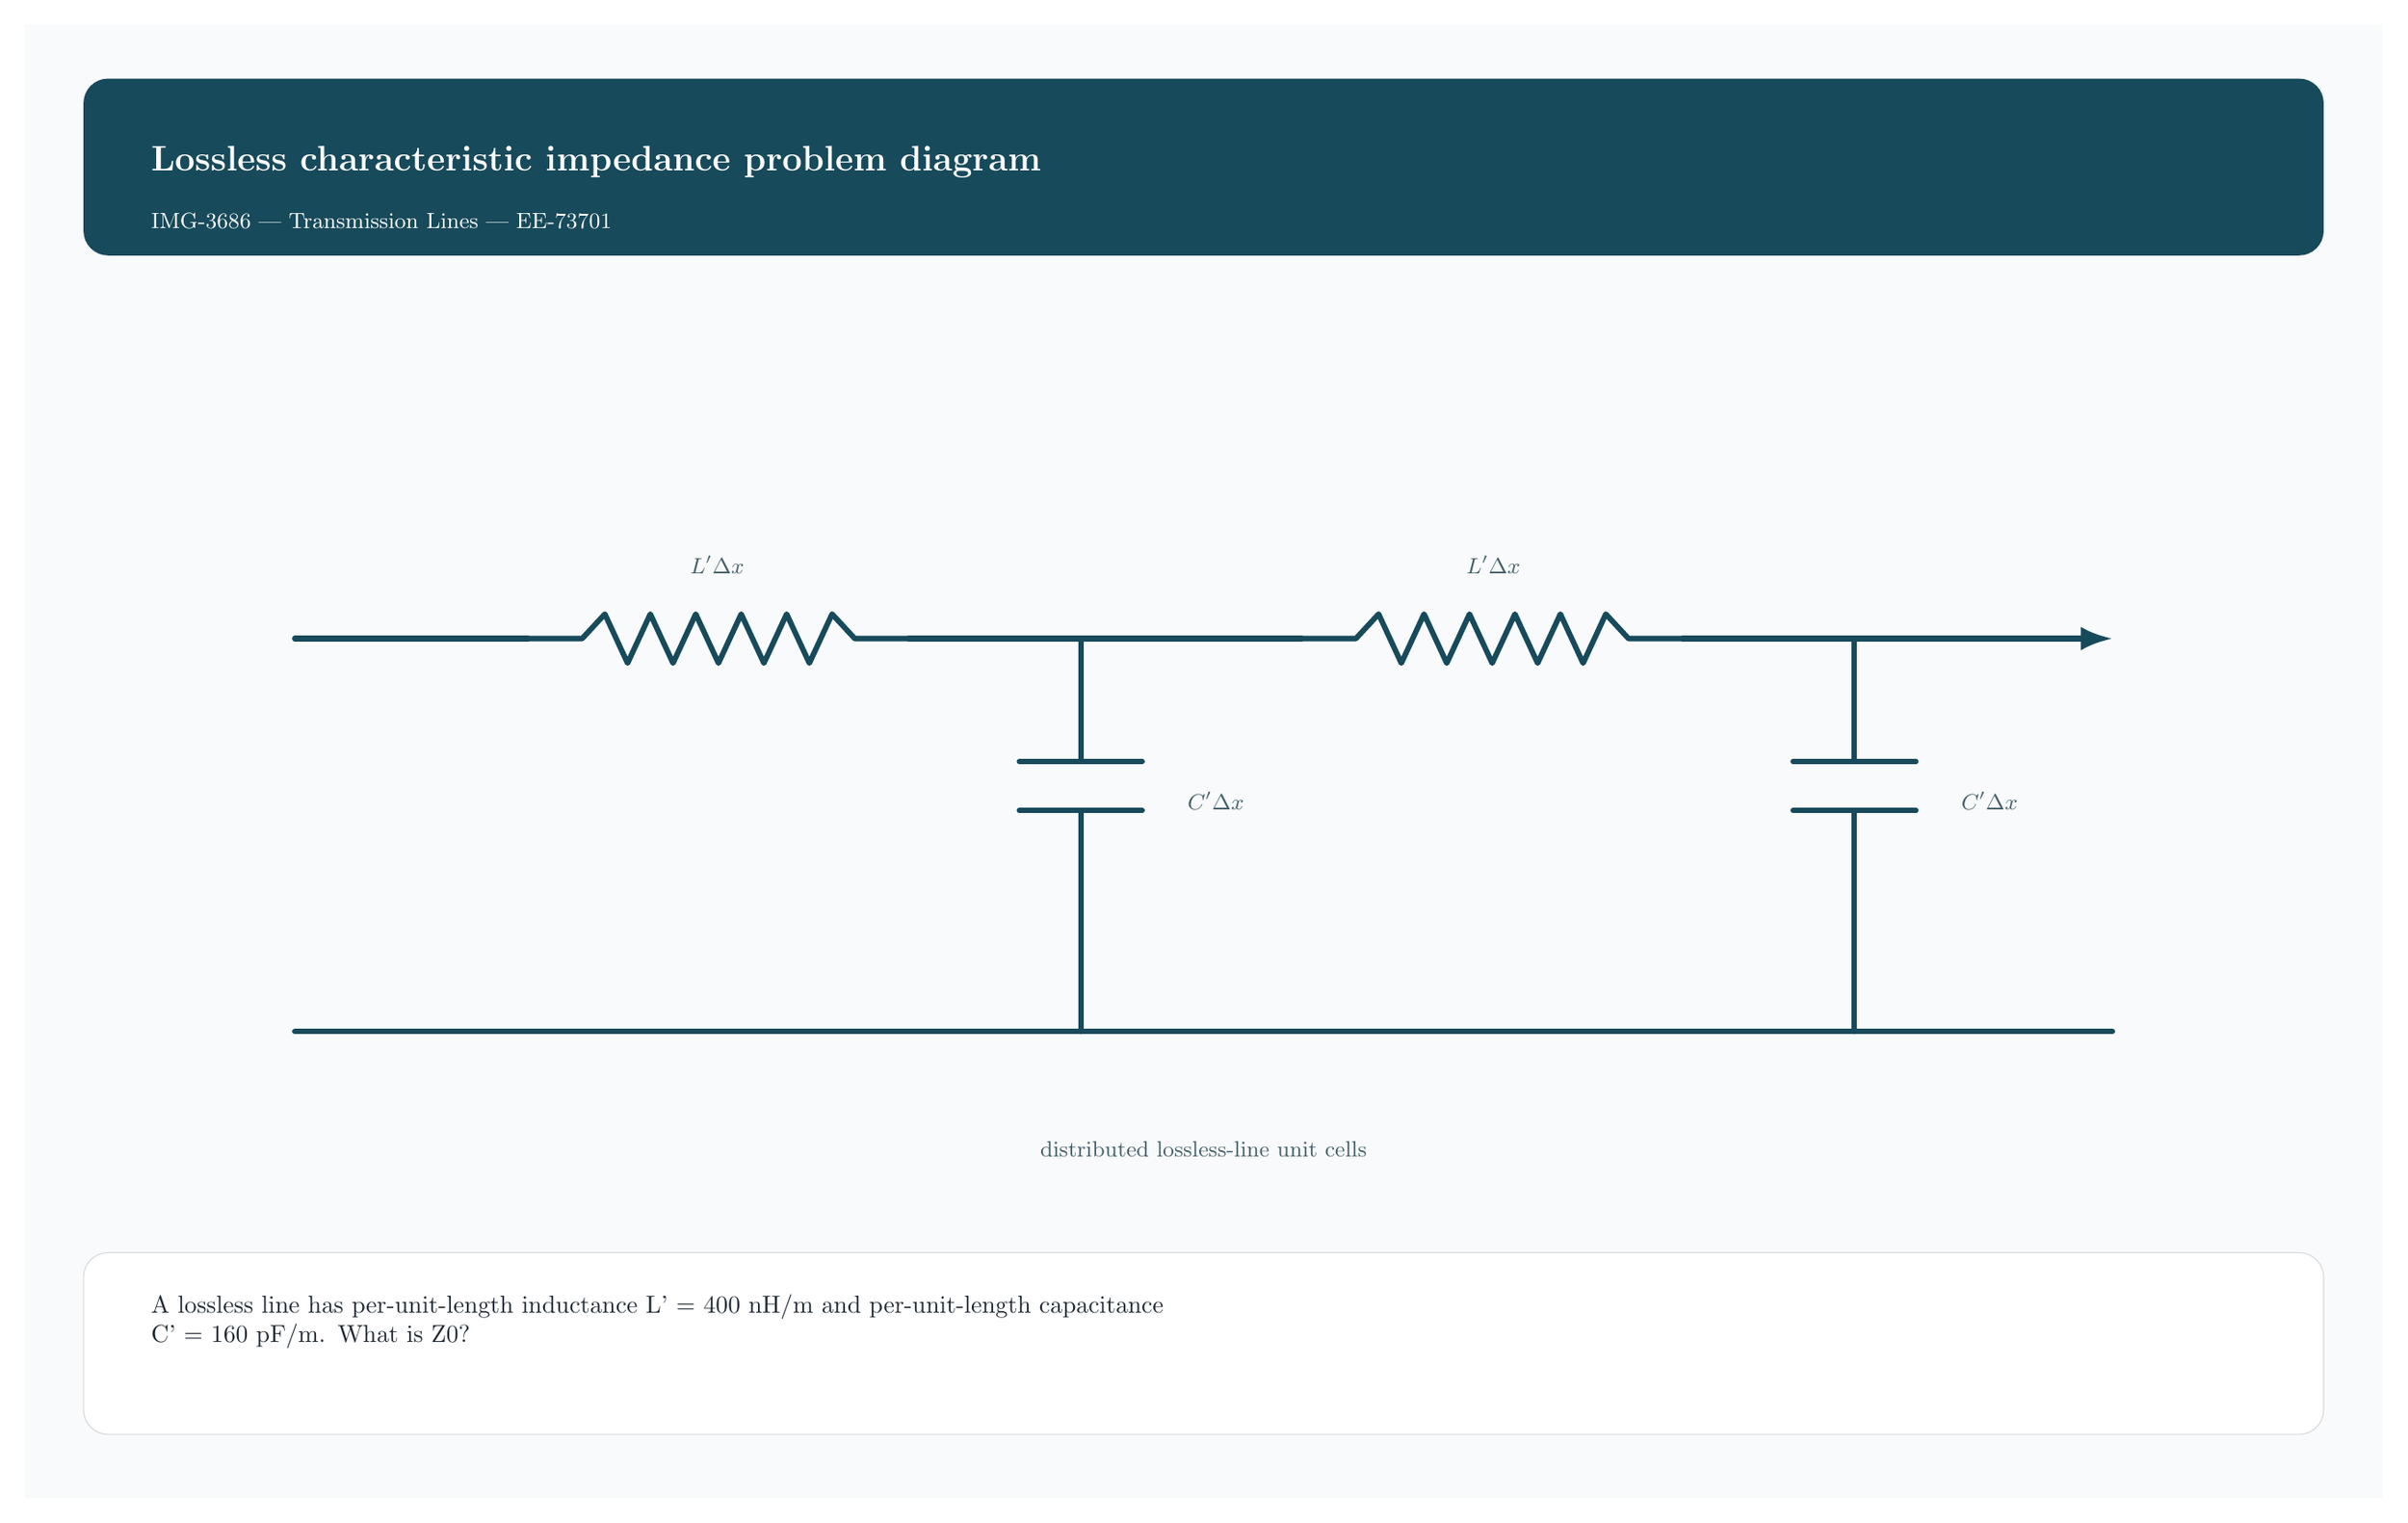
\begin{tikzpicture}[x=1pt,y=-1pt,>=Latex,line cap=round,line join=round]
\path[fill=zyloPaper] (0,0) rectangle (960,600);
\path[fill=zyloTeal,rounded corners=10pt] (24,22) rectangle (936,94);
\node[anchor=west,text=white,font=\bfseries\Large] at (48,56) {Lossless characteristic impedance problem diagram};
\node[anchor=west,text=white!82,font=\small] at (48,80) {IMG-3686 | Transmission Lines | EE-73701};
\tikzset{wire/.style={draw=zyloTeal,line width=2.2pt},thinwire/.style={draw=zyloLine,line width=1.35pt},accent/.style={draw=zyloOrange,line width=2.2pt},box/.style={draw=zyloTealTwo,fill=zyloSoft,line width=1.5pt,rounded corners=8pt}}
\draw[wire] (110,250) -- (205,250);
\draw[wire] (205,250) -- (227,250) -- (227,250) -- (236.25,240) -- (245.5,260) -- (254.75,240) -- (264,260) -- (273.25,240) -- (282.5,260) -- (291.75,240) -- (301,260) -- (310.25,240) -- (319.5,260) -- (328.75,240) -- (338,250) -- (360,250);
\draw[wire] (360,250) -- (520,250);
\draw[wire] (520,250) -- (542,250) -- (542,250) -- (551.25,240) -- (560.5,260) -- (569.75,240) -- (579,260) -- (588.25,240) -- (597.5,260) -- (606.75,240) -- (616,260) -- (625.25,240) -- (634.5,260) -- (643.75,240) -- (653,250) -- (675,250);
\draw[wire,->] (675,250) -- (850,250); \draw[wire] (110,410) -- (850,410);
\draw[wire] (430,250) -- (430,300); \draw[wire] (405,300) -- (455,300); \draw[wire] (405,320) -- (455,320); \draw[wire] (430,320) -- (430,410);
\draw[wire] (745,250) -- (745,300); \draw[wire] (720,300) -- (770,300); \draw[wire] (720,320) -- (770,320); \draw[wire] (745,320) -- (745,410);
\node[font=\small,text=zyloLine] at (282,220) {$L'\Delta x$}; \node[font=\small,text=zyloLine] at (598,220) {$L'\Delta x$};
\node[font=\small,text=zyloLine] at (485,316) {$C'\Delta x$}; \node[font=\small,text=zyloLine] at (800,316) {$C'\Delta x$};
\node[font=\small,text=zyloLine] at (480,458) {distributed lossless-line unit cells};
\path[draw=black!15,fill=white,rounded corners=10pt] (24,500) rectangle (936,574);
\node[anchor=west,text width=860pt,align=left,text=zyloInk,font=\normalsize] at (48,528) {A lossless line has per-unit-length inductance L' = 400 nH/m and per-unit-length capacitance\\C' = 160 pF/m. What is Z0?};
\end{tikzpicture}
\end{document}
